\documentclass[a4paper,10pt]{article}
\usepackage[utf8]{inputenc}
\usepackage[T1]{fontenc}
\usepackage{graphicx}
\graphicspath{ {./} }
\usepackage[MeX]{polski}

%opening
\title{Angielski 04}
\author{}

\begin{document}

\maketitle

\begin{abstract}
Na przyszły tydzień: \\
U1 glending Information Technology (1)\\
U1 (2) proffesional languane for ... \\

Materiały: \\
https://sandymillin.wordpress.com/2011/05/01/describing-graphs/ \\

\end{abstract}

\subsection{Describing a graph}
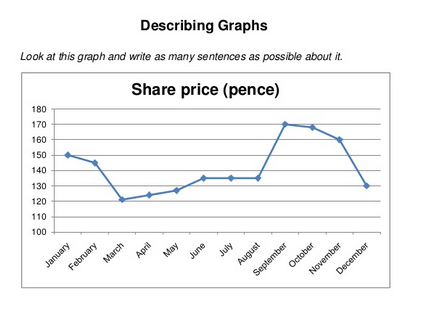
\includegraphics[width=\textwidth]{ang-2019-11-07-describe.png} \\
In January the share price was 150 pence. In February and March it fell, finishing at 120. After that it fell gradually gained till June, reaching 123 in April, 127 in May and 135 in June. Form June till August it stayed (?) still. In September it rose to 170, after which it fell till the end of the year, reaching 168 in October, 160 in November and closing the year with a dramatic drop to 130 pence.

\section{Present Perfect vs Simple Past}
Simple Past-dookreślony czas (when?, yesterday, date). \\
Present Perfect-Recently, lately, so far, never, ever \\
\\
You lived in Poznań vs You've lived in Poznań.\\


\section{Homework}
historic vs historical, how to rememebr the difference \\
strona 28 z business presentations

\end{document}
